\documentclass[a4paper]{article}

\usepackage{url}
\usepackage{amsmath}
\usepackage{verbatim}   		% Useful for program listings
\usepackage[T1]{fontenc}       	% For Swedish characters ÅÄÖ etc.
\usepackage[utf8]{inputenc}
% \usepackage[swedish]{babel} % For Swedish hyphenation
\usepackage{fancyvrb}           	% For lists with tabulators
\fvset{tabsize=4}              	 	% Tabulator size
\fvset{fontsize=\small}         	% List font size
\usepackage{graphicx}		% Imports the graphicx package, useful for images

% generate clickable references & toc
\usepackage[]{hyperref}
\hypersetup{
%    pdftitle={Your title here},
%    pdfauthor={Your name here},
%    pdfsubject={Your subject here},
%    pdfkeywords={keyword1, keyword2},
    bookmarksnumbered=true,
    bookmarksopen=true,
    bookmarksopenlevel=1,
    colorlinks=true,
    pdfstartview=Fit,
    pdfpagemode=UseOutlines,    % this is the option you were lookin for
    pdfpagelayout=TwoPageRight
}

% \usepackage{}

\title{Dragonfly System Software Design}
\author{Daniel Stenberg \\ Adam Steineck}

\date{\today}         		% Today's date if not specified

\begin{document}                	% Start of document

\maketitle                      		% Prints the title defined above with \title, \author and \date

\begin{center}
\vspace{64pt}

\includegraphics[scale=1.6]{images/AF_Logotype20141_Black.png}
\vspace{16pt}
\\ \large ÅF Embedded Systems
\end{center}

\newpage

\tableofcontents				% Insert table of contents

\newpage

\section{General}

The \emph{Dragonfly} project is an internal competence enhancement project for ÅF employees. The goal is to combine technology, competence and experience from various engineering fields in order to construct a highly advanced quadrotor UAV system.

\subsection{Introduction}
This document is a technical description of the design aspects DragonFly. These are:
\begin{itemize}
\item Bot CPU to Flight Dynamics CPU
\item Bot CPU to App SW
\end{itemize}

\subsection{Scope}
This document is intended for engineers involved with developing, designing and maintaining the Dragonfly Project. For editors of this document, see section \ref{sec:editors}.

\subsection{Information to Document Editors}
\label{sec:editors}
This PDF document was created with \LaTeX and uses UK English spelling conventions. Its \texttt{.tex} source is in repo \url{https://github.com/afconsult-south/dragonfly} directory \texttt{doc}.

\subsection{Document Change Log}
Reverse chronological order.

\begin{center}
\begin{tabular}{ c | l }
  \hline
  Version & Version description. \\ \hline
   & put next version here. \\ \hline
  v0.0 & Work in progress - first draft. \\ \hline
\end{tabular}
\end{center}

\newpage

\section{System description}
The quadcopter will have autonomous behaviour, for instance to avoid collisions, land automatically and to be able to recharge itself by docking with a charging station.

There is a requirement list for the DragonFly Quadcopter somewhere TODO link.

\begin{figure}[!h]
    \centering
    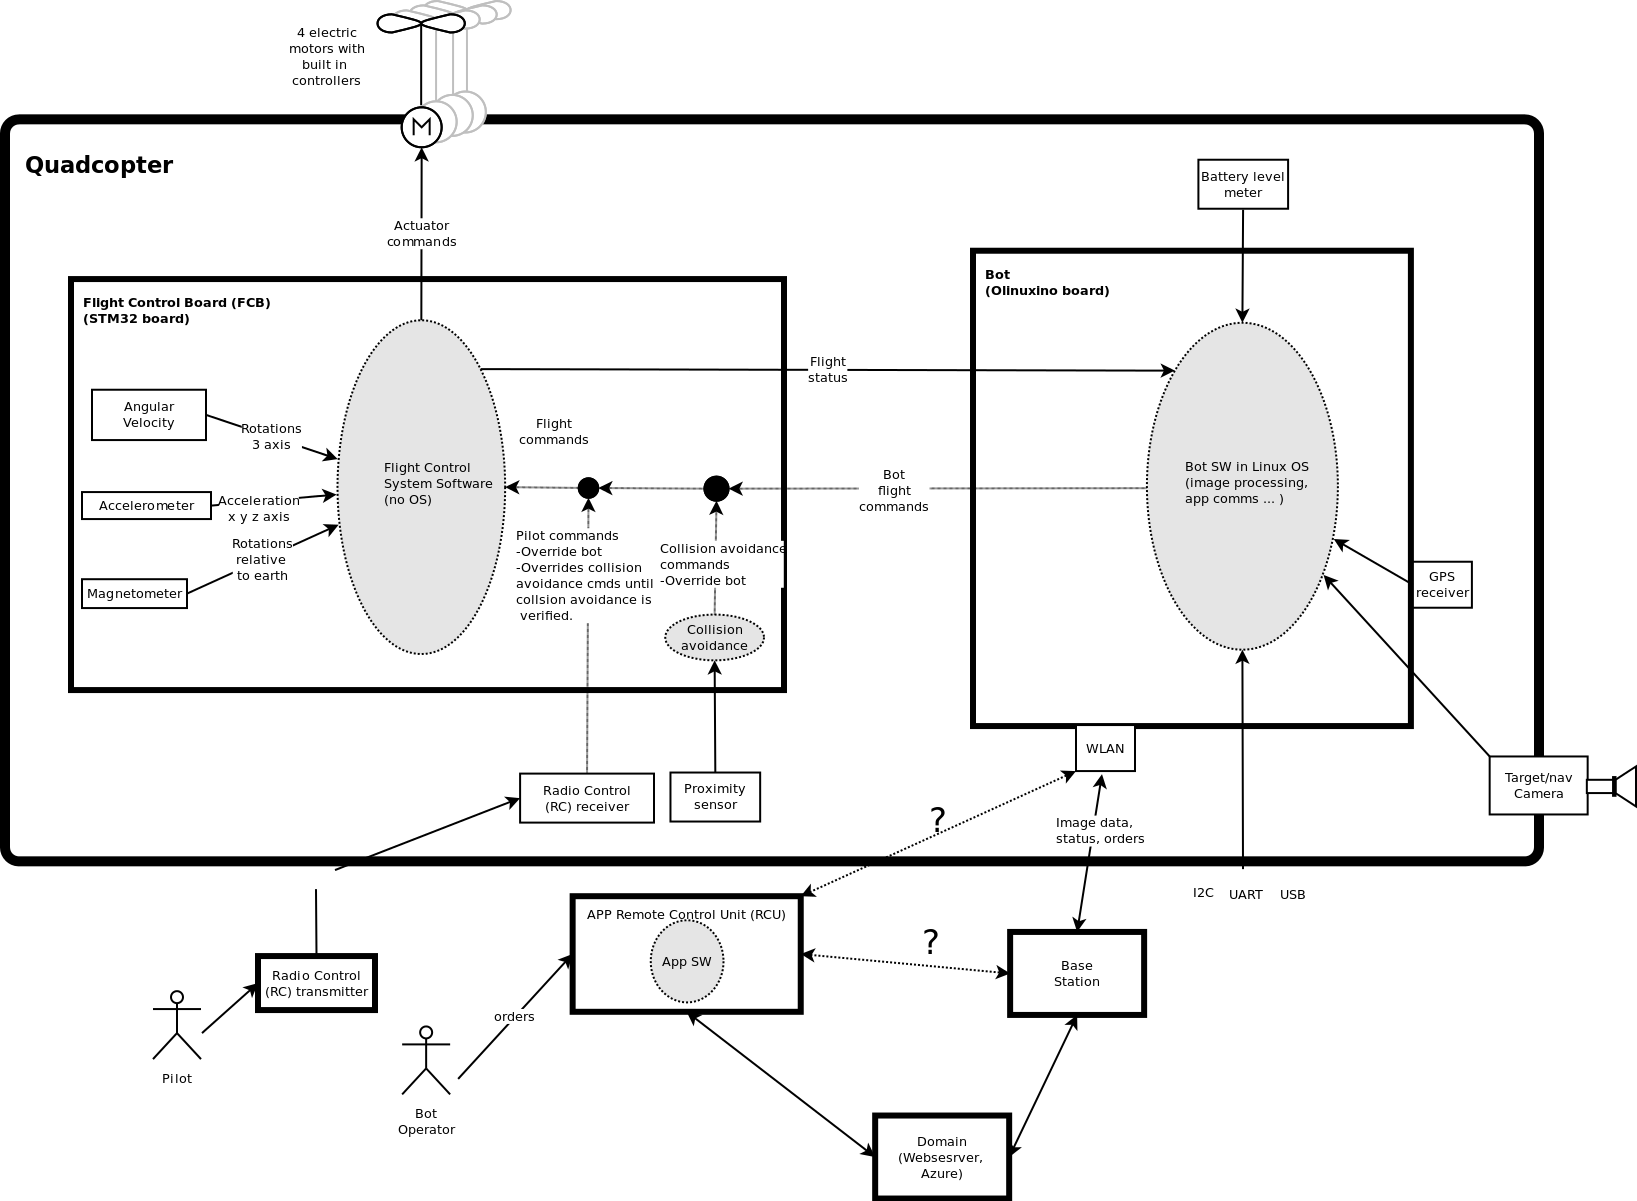
\includegraphics[width=\textwidth]{images/SystemArchitectureDiagram_DF.png}
    \caption{SystemArchitectureDiagram}
    \label{fig:sysarchdiag}
\end{figure}

\section{Flight Software (Flight Control Board)}
The quadcopter is self-stabilising which is handled by the Flight Control Board.

  \subsection{Flight commands}
  These commands provide the set point for the flight control software.
  \subsubsection{Definition}
  \label{sec:flightcmd-definition}
  \begin{itemize}
    \item Rotational commands (as viewed from above)
      \begin{itemize}
        \item Rotate clockwise.
        \item Rotate anticlocwise.
      \end{itemize}
      \item Translational commands
        \begin{itemize}
          \item Forward
          \item Backward
          \item Slide left
          \item Slide right
        \end{itemize}
  \end{itemize}

  \subsubsection{Sources of flight commands}
  \label{sec:flight-cmd-src}
  Flight commands may come from, in order of priority:
  \begin{enumerate}
    \item A competent pilot using the R/C radio TX.
    \item Collision avoidance functionality in Flight Control Board.
    \item Autonomous Bot SW in automatic navigation.
    \item The Bot Operator using the App SW.
  \end{enumerate}
  Automatic navigation involves either following a set flight path or exploratory mode using the navigation camera.

  \subsubsection{Flight Control Theory}
  See reference \cite{fcb}.

  \subsubsection{Flight sensor inputs}
  \label{sec:flight-sensor-inputs}
  The Flight Control Board has sensors which monitor:
  \begin{itemize}
    \item Acceleration along all three geometric axes.
    \item Rotational velocity around all three geometric axes.
    \item A compass which measures rotation relative to Earth's magnetic field
    \item Proximity sensors measuring distance to nearest object in all 3 axis, a total of six sensors. The forward-facing sensor should have greater range, see section \ref{sec:collision-avoidance}. The bottom sensor needs enough precision to allow docking on the charging station.
  \end{itemize}
  \subsubsection{Collision avoidance}
  \label{sec:collision-avoidance}
  Collision avoidance is calculated in the Flight Dynamics processor. This is a safety feature designed to decrease the risk of injury to either humans, damage to surrounding objects or the quad-copter itself. This is thus the only source of set point flight control inputs which originate inside the Flight Dynamics processor. The forward proximity sensor need greater range than the others as to give a sufficiently long braking distance. The forward sensor determines the available braking distance and top velocity will have to be low enough to allow coming to a full stop inside this distance at all times.

  When collision avoidance is guiding the quadrotor, this status is sent to Bot SW.

\section{Flight Management Software (FMS) subsystem}
This subsystem governs autonomous behaviour, payload and communication with App SW.

  \subsection{Autonomous behaviour}
  The autonomous behaviour of Dragonfly is realised by an autopilot built into Bot SW.

  \subsubsection{Battery monitor}
  The Bot SW monitors the battery level so a return journey to the charging station can be planned in a timely manner.

  \subsubsection{Camera navigation}
  \begin{itemize}
    \item \textbf{Explore:} With the camera, Dragonfly will be able to map a room and should be able to negotiate open doors.
    \item \textbf{Follow moving object:} With the help of a camera, Dragonfly will be able to follow a moving object around.
  \end{itemize}

  \subsubsection{Follow set flight path}
  App SW may dictate a flight path. FCB listens to App SW commands listed in section \ref{sec:flightcmd-definition}.
  \subsection{Payload}
  Bot SW and the load carrying capacity of Dragonfly allows a USB device to be carried as payload. Bot SW will handle the interface to this device.
  \subsection{Status transmission}
  Bot SW sends status from itself and forwards status from Flight SW to App SW.

\section{App SW}
This allows the Bot Operator via a HMI to monitor \& control the quad-copter:
\begin{itemize}
\item Monitor status as in section \ref{sec:fms-status-2-app}.
\item To issue instructions as in section \ref{sec:app-cmds-2-fms}.
\item Display live camera feed from navigation camera.
\item Display feed from USB payload camera.
\end{itemize}

\section{Inter subsystem communication}
This section is a technical overview of communication interfaces in DragonFly. These are:
\begin{itemize}
  \item Flight Control Board (FCB) to Flight Management System (FMS)
  \item FMS to App SW.
 \end{itemize}

\subsection{FMS to FCB}

\subsubsection{Initiation}
\begin{itemize}
\item FCB waits for FMS to connect.
\item Flight dynamics data is pushed to FMS periodically without prompting.
\item FCB expects incoming flight commands.
\end{itemize}

\subsubsection{Flight Status feedback to Bot SW}
\begin{itemize}
\item Sensor inputs as outlined in section \ref{sec:flight-sensor-inputs}.
\item Current source of flight command as per section \ref{sec:flight-cmd-src}.
\end{itemize}


\subsection{App SW to FMS communication}
\subsubsection{Initiation}
\begin{itemize}
\item Bot SW indefinitely waits for App SW to connect.
\item Upon connection, Bot SW will push flight data to App SW without prompting and expect incoming flight commands.
\end{itemize}
\subsubsection{FMS status to App SW}
\label{sec:fms-status-2-app}
\begin{itemize}
\item Rotational acceleration parameters
\item Linear acceleration parameters
\item Flight Dynamics control status (R/C Pilot, Collision Avoidance, Bot SW or App SW)
\item Camera status (Disabled, Active, In Use)
\item Battery status
\item Other hardware configuration
\item GPS coordinates
\end{itemize}
\subsubsection{Instructions from App SW to FMS}
\label{sec:app-cmds-2-fms}
\begin{itemize}
\item A flight path to follow for Bot SW autopilot, in delta position or GPS coordinates.
\item In absolute GPS coordinates.
\item Direct control (up, down, left, right rotate CW, rotate ACW)
\item Flight path to follow
\item Return to docking station.
\item Land
\item Follow object
\end{itemize}
\subsubsection{Camera video stream}
The video stream from the navigation camera should be available to App SW.

\subsubsection{Payload management}
App SW should be able to receive a camera stream from a carried camera.

\begin{thebibliography}{99}
\bibitem[1]{stenberg} Model-based Design Development and Control of a Wind Resistant Multirotor UAV, C. Månsson, D. Stenberg, Lunds Tekniska Högskola 2014
\bibitem[2]{fcb} Dragonfly Flight Control Board, D. Stenberg ÅF.
\end{thebibliography}

\end{document}
